\documentclass{article}
\usepackage[T1]{fontenc}
\usepackage{lmodern}
\usepackage{graphicx}
\usepackage{amsmath,amssymb}
\usepackage[a4paper,margin=2cm]{geometry}
\usepackage[absolute,overlay]{textpos}
\setlength{\TPHorizModule}{1mm}
\setlength{\TPVertModule}{1mm}
\usepackage[indonesian]{babel}
\usepackage{hyperref}
\setlength{\emergencystretch}{2em}
% unit: Halaman 43

\begin{document}

% === Halaman 43 (llm) ===

\vspace{178.20mm}

Sumber: \url{https://www.semanticscholar.org/paper/Acoustic-Eavesdropping-through-Wireless-Vibrometry-Wei-Wang/8afd80726c54ed7b95d30d1230bef633d128c930}

% deskripsi: Ilustrasi dua skenario penyadapan akustik: (kiri) metode Reflective menggunakan pengirim (Tx) dan penerima (Rx) untuk mendeteksi getaran dari speaker korban, dan (kanan) metode Emissive menggunakan AP dan penerima (Rx) untuk mendeteksi emisi dari smartphone korban melalui dinding.
% bbox normalisasi: [0.1500, 0.1400, 0.8400, 0.7400]
\begin{textblock*}{144.90mm}(31.50mm,41.58mm)
\noindent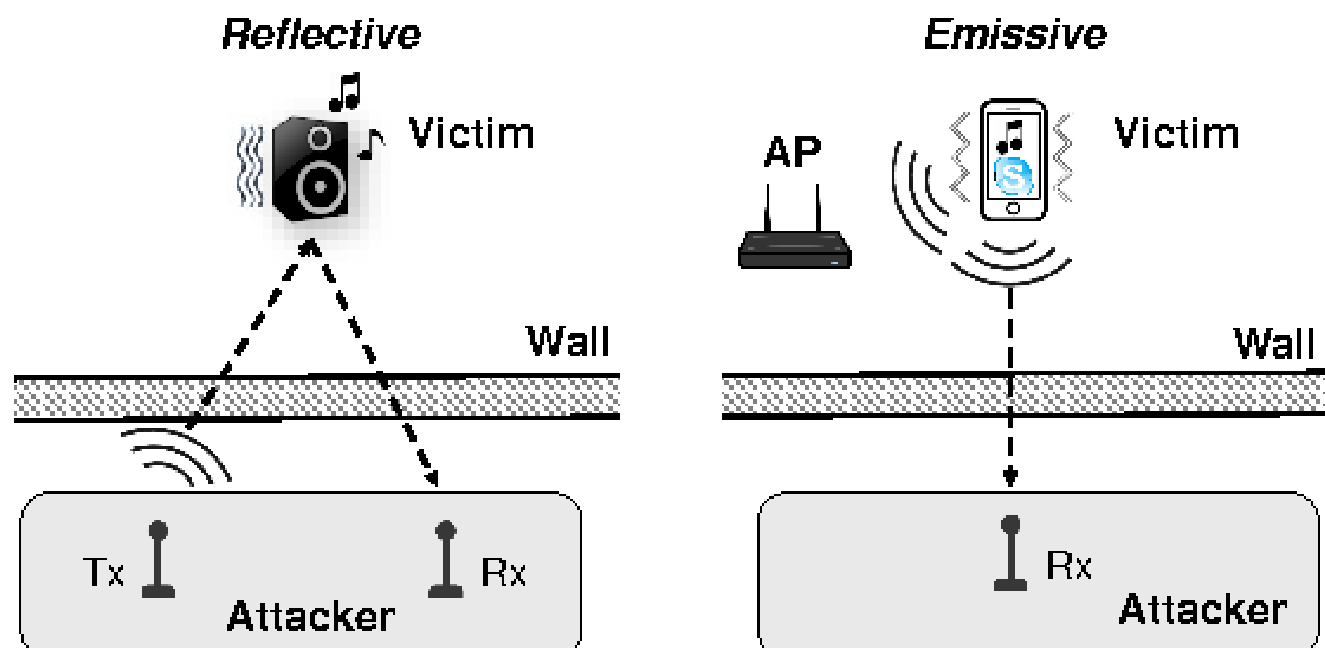
\includegraphics[width=144.90mm,height=178.20mm]{../../images/llm/page_043_img_01.png}%
\end{textblock*}

\end{document}
